\documentclass[tikz,border=10pt]{standalone}
\usetikzlibrary{calc}
\begin{document}
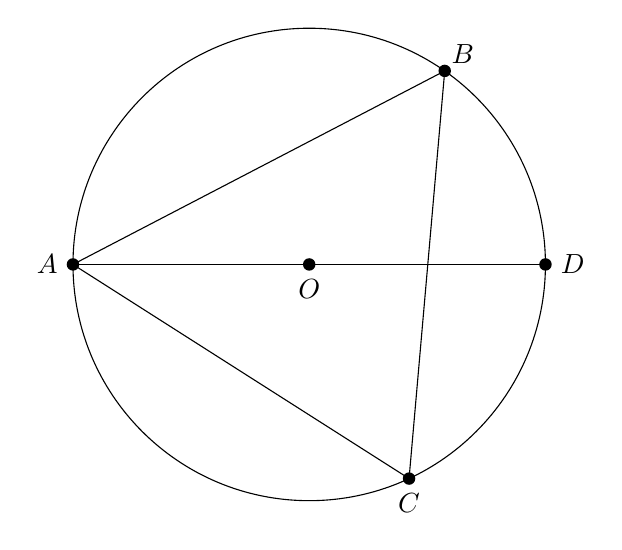
\begin{tikzpicture}[scale=1.5]
  \coordinate (O) at (0,0);
  \coordinate (A) at (-2,0);
  \coordinate (D) at (2,0);
  \coordinate (B) at (55:2);
  \coordinate (C) at (-65:2);
  \draw (O) circle (2);
  \draw (A) -- (D);
  \draw (A) -- (B);
  \draw (A) -- (C);
  \draw (B) -- (C);
  \fill (O) circle (1.5pt);
  \fill (A) circle (1.5pt);
  \fill (B) circle (1.5pt);
  \fill (C) circle (1.5pt);
  \fill (D) circle (1.5pt);
  \node[below=2pt] at (O) {$O$};
  \node[left=2pt] at (A) {$A$};
  \node[above right=-1pt] at (B) {$B$};
  \node[below=2pt] at (C) {$C$};
  \node[right=2pt] at (D) {$D$};
\end{tikzpicture}
\end{document}
